\appendix
\label{sec:appendix}
\section{Workflow-Specific Execution Results of Baseline and Co-location Algorithms}
\begin{figure}[H]
    \centering
    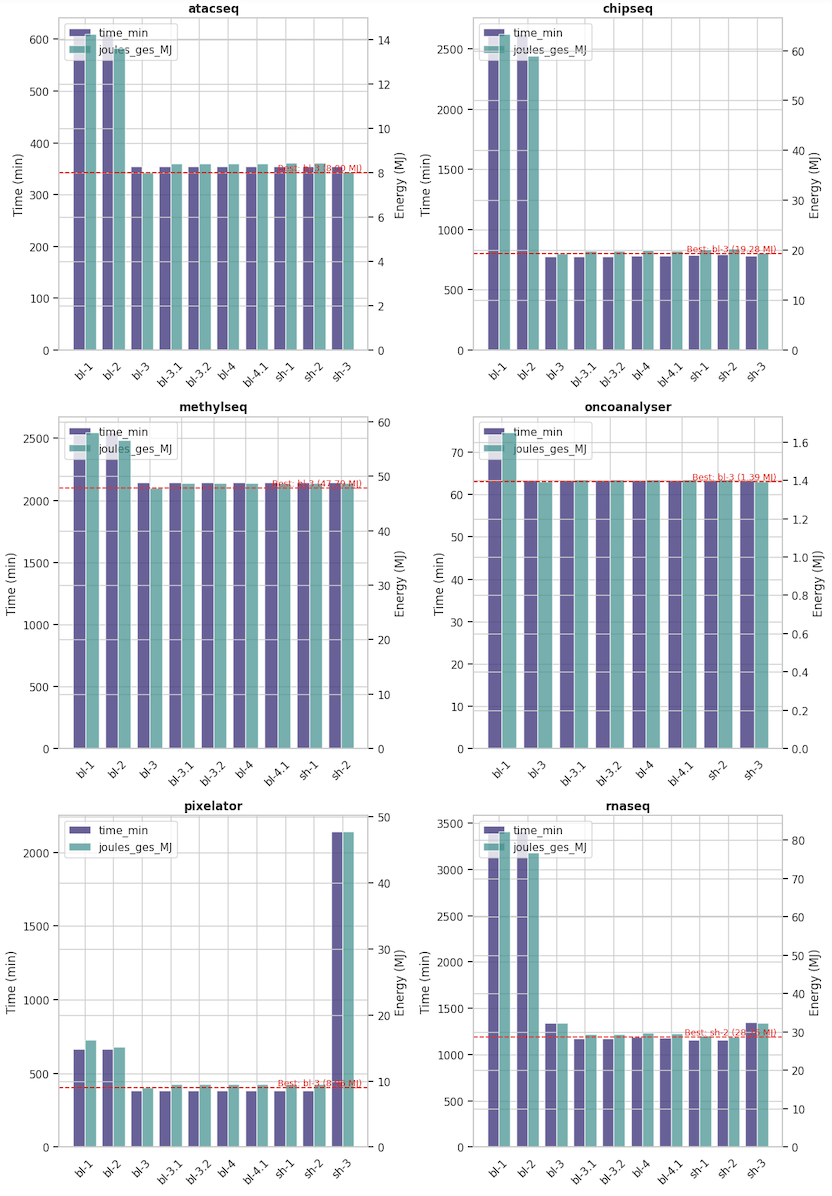
\includegraphics[scale=0.8]{fig/09/09_appendiy_1.png}
    \small
    \caption{Execution Results of Baseline and Co-location Algorithms}
    \label{fig:09-rf}
    \tiny
    Execution Results of Baseline and Co-location Algorithms
\end{figure}
\begin{figure}[H]
    \centering
    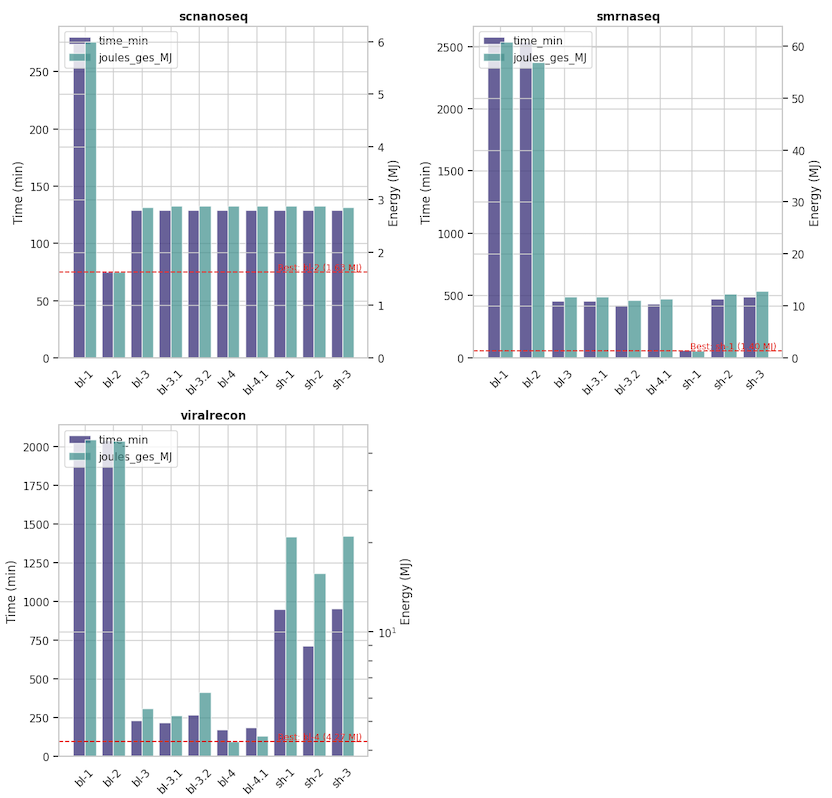
\includegraphics[scale=0.8]{fig/09/09_appendix_2.png}
    \small
    \caption{Execution Results of Baseline and Co-location Algorithms}
    \label{fig:09-rf}
    \tiny
    Execution Results of Baseline and Co-location Algorithms
\end{figure}
\section{Blueprint Baseline Algorithms for the \textit{ShaRiff} Approach}

% Baseline 1

\begin{algorithm}[H]
    \caption{Baseline~1 — FIFO Scheduling with Round-Robin Host Assignment}
    \label{alg:baseline1_refined}
    \KwIn{workflow \( G=(T,E) \), hosts \( \mathcal{H} = \{h_1,\dots,h_m\} \)}
    \KwOut{each task \( t_i \in T \) executed once all dependencies are resolved}

    \BlankLine
    Initialize idle cores \( c(h_j) \gets C_j \) for all \( h_j \in \mathcal{H} \)
    Initialize empty ready queue \( \mathcal{Q} \)
    Enqueue all source tasks (no predecessors) into \( \mathcal{Q} \) in FIFO order
    Set host index \( k \gets 1 \)

    \BlankLine
    \While{not all tasks \( t_i \in T \) completed}{
        \While{\( \mathcal{Q} \) not empty}{
            Let \( t_i \) be the head of \( \mathcal{Q} \)
            Select host \( h_k \) in round-robin order from \( \mathcal{H} \)
            \If{\( c(h_k) > 0 \)}{
                Reserve one core: \( c(h_k) \gets c(h_k) - 1 \)
                Launch VM \( v = (1,\, M_{t_i},\, h_k) \) to execute \( t_i \)
                Dequeue \( t_i \) from \( \mathcal{Q} \)
            }
            Advance to next host index \( k \gets (k \bmod m) + 1 \)
        }
        Wait until a running task \( t_r \) completes
        Release its host core: \( c(h(t_r)) \gets c(h(t_r)) + 1 \)
        For each successor \( t_s \) of \( t_r \), enqueue \( t_s \) into \( \mathcal{Q} \) if all predecessors are completed
    }
    \Return{workflow complete}
\end{algorithm}

% Baseline 2
\begin{algorithm}[H]
    \caption{Baseline~2 — FIFO Scheduling with Host Backfilling}
    \label{alg:baseline2_refined}
    \KwIn{workflow \( G=(T,E) \), hosts \( \mathcal{H} = \{h_1,\dots,h_m\} \)}
    \KwOut{each task \( t_i \in T \) executed once all dependencies are resolved}

    \BlankLine
    Initialize idle cores \( c(h_j) \gets C_j \) for all \( h_j \in \mathcal{H} \)
    Initialize empty ready queue \( \mathcal{Q} \)
    Enqueue all source tasks (no predecessors) into \( \mathcal{Q} \) in FIFO order

    \BlankLine
    \While{not all tasks \( t_i \in T \) completed}{
        \While{\( \mathcal{Q} \) not empty}{
            Let \( t_i \) be the head of \( \mathcal{Q} \)
            Find the first host \( h_j \in \mathcal{H} \) with \( c(h_j) > 0 \)
            \If{such \( h_j \) exists}{
                Reserve one core: \( c(h_j) \gets c(h_j) - 1 \)
                Launch VM \( v = (1,\, M_{t_i},\, h_j) \) to execute \( t_i \)
                Dequeue \( t_i \) from \( \mathcal{Q} \)
            }
            \Else{
                \textbf{break}  \tcp*[r]{no idle host available, defer assignment}
            }
        }
        Wait until a running task \( t_r \) completes
        Release its core: \( c(h(t_r)) \gets c(h(t_r)) + 1 \)
        For each successor \( t_s \) of \( t_r \), enqueue \( t_s \) into \( \mathcal{Q} \) if all predecessors are completed
    }
    \Return{workflow complete}
\end{algorithm}

% Baseline 3
\newpage
\begin{algorithm}[H]
    \caption{Baseline~3 — FIFO Scheduling with VM Co-Location}
    \label{alg:baseline3_refined}
    \KwIn{workflow \( G=(T,E) \), hosts \( \mathcal{H} = \{h_1,\dots,h_m\} \)}
    \KwOut{all tasks \( t_i \in T \) executed, with ready tasks co-located on shared VMs when possible}

    \BlankLine
    Initialize idle cores \( c(h_j) \gets C_j \) for all \( h_j \in \mathcal{H} \)
    Initialize empty ready queue \( \mathcal{Q} \)
    Enqueue all source tasks (no predecessors) into \( \mathcal{Q} \) in FIFO order

    \BlankLine
    \While{not all tasks \( t_i \in T \) completed}{
        \While{\( \mathcal{Q} \) not empty}{
            Find first host \( h_j \) with \( c(h_j) > 0 \)
            \If{no such host exists}{
                \textbf{break}  \tcp*[r]{wait for resource release}
            }
            Select subset \( \mathcal{T}_j \subseteq \mathcal{Q} \) such that
            \(\text{sum(req\_cores}(\mathcal{T}_j)) \le c(h_j)\)
            Allocate VM \( v_j = (\text{sum(req\_cores}(\mathcal{T}_j)),\, \text{sum(req\_mem}(\mathcal{T}_j)),\, h_j) \)\\
            Launch all tasks \( t_i \in \mathcal{T}_j \) on \( v_j \)
            Update \( c(h_j) \gets c(h_j) - \text{cores}(v_j) \) and remove \( \mathcal{T}_j \) from \( \mathcal{Q} \)
        }
        Wait until a task \( t_r \) completes
        Release its cores: \( c(h(t_r)) \gets c(h(t_r)) + \text{req\_cores}(t_r) \)
        \If{all tasks on \( v_j \) finished}{
            Destroy VM \( v_j \)
        }
        For each successor \( t_s \) of \( t_r \), enqueue \( t_s \) into \( \mathcal{Q} \) if all predecessors are completed
    }
    \Return{workflow complete}
\end{algorithm}
% Baseline 3.1
\begin{algorithm}[H]
    \caption{Baseline~3.1 — FIFO Scheduling with Max-Core VM Co-Location}
    \label{alg:baseline3.1_refined}
    \KwIn{workflow \( G=(T,E) \), hosts \( \mathcal{H} = \{h_1,\dots,h_m\} \)}
    \KwOut{all tasks \( t_i \in T \) executed, co-located on VMs at hosts with maximum idle capacity}

    \BlankLine
    Initialize idle cores \( c(h_j) \gets C_j \) for all \( h_j \in \mathcal{H} \)
    Initialize empty ready queue \( \mathcal{Q} \)
    Enqueue all source tasks (no predecessors) into \( \mathcal{Q} \) in FIFO order

    \BlankLine
    \While{not all tasks \( t_i \in T \) completed}{
        \While{\( \mathcal{Q} \) not empty}{
            Select host \( h_j = \arg\max_{h \in \mathcal{H}} c(h) \)
            \If{\( c(h_j) = 0 \)}{
                \textbf{break}  \tcp*[r]{no host available, wait for completion}
            }
            Select subset \( \mathcal{T}_j \subseteq \mathcal{Q} \) such that
            \(\text{sum(req\_cores}(\mathcal{T}_j)) \le c(h_j)\)
            Allocate VM \( v_j = (\text{sum(req\_cores}(\mathcal{T}_j)),\, \text{sum(req\_mem}(\mathcal{T}_j)),\, h_j) \)\\
            Launch all tasks \( t_i \in \mathcal{T}_j \) on \( v_j \)
            Update \( c(h_j) \gets c(h_j) - \text{cores}(v_j) \) and remove \( \mathcal{T}_j \) from \( \mathcal{Q} \)
        }
        Wait until a task \( t_r \) completes
        Release its resources: \( c(h(t_r)) \gets c(h(t_r)) + \text{req\_cores}(t_r) \)
        \If{all tasks on \( v_j \) finished}{
            Destroy VM \( v_j \)
        }
        For each successor \( t_s \) of \( t_r \), enqueue \( t_s \) into \( \mathcal{Q} \) if all predecessors are completed
    }
    \Return{workflow complete}
\end{algorithm}
% Baseline 3.2
\newpage
\begin{algorithm}[H]
    \caption{Baseline~3.2 — FIFO Scheduling with Max-Parallel VM Co-Location}
    \label{alg:baseline3.2_refined}
    \KwIn{workflow \( G=(T,E) \), hosts \( \mathcal{H}=\{h_1,\dots,h_m\} \)}
    \KwOut{all tasks \( t_i\in T \) executed with host-level parallel assignment and intra-host co-location}

    \BlankLine
    Initialize idle cores \( c(h_j)\gets C_j \) for all \( h_j\in\mathcal{H} \)
    Initialize empty ready queue \( \mathcal{Q} \)
    Enqueue all source tasks (no predecessors) into \( \mathcal{Q} \) in FIFO order

    \BlankLine
    \While{not all tasks \( t_i\in T \) completed}{
        Build available-host list \( L = \{\,h \in \mathcal{H}\mid c(h)>0\,\} \), sorted by \( c(h) \) descending\\
        \If{\( L \) is empty}{
            Wait for any running task to finish; update \( c(\cdot) \); \textbf{continue}
        }
        Initialize empty host-batch mapping set \( \mathcal{M} \)
        \ForEach{host \( h \in L \) \textbf{and} while \( \mathcal{Q} \) not empty}{
            Select subset \( \mathcal{T}_h \subseteq \mathcal{Q} \) in FIFO order such that \(\text{sum(req\_cores}(\mathcal{T}_h)) \le c(h)\)\\
            \If{\( \mathcal{T}_h \neq \emptyset \)}{
                Add mapping \( (h,\mathcal{T}_h) \) to \( \mathcal{M} \)
            }
        }

        \ForEach{mapping \( (h,\mathcal{T}_h) \in \mathcal{M} \)}{
            Allocate VM \( v_h = (\text{sum(req\_cores}(\mathcal{T}_h)),\, \text{sum(req\_mem}(\mathcal{T}_h)),\, h) \)\\
            Launch all \( t \in \mathcal{T}_h \) on \( v_h \)
            Update \( c(h) \gets c(h) - \text{cores}(v_h) \) and remove \( \mathcal{T}_h \) from \( \mathcal{Q} \)
        }

        Wait until any task \( t_r \) completes
        Release its cores: \( c(h(t_r)) \gets c(h(t_r)) + \text{req\_cores}(t_r) \)
        \If{its VM \( v_h \) has no active tasks}{Destroy \( v_h \)}
        For each successor \( t_s \) of \( t_r \), enqueue \( t_s \) into \( \mathcal{Q} \) if all predecessors have completed
    }
    \Return{workflow complete}
\end{algorithm}
% Baseline 4
\begin{algorithm}[H]
    \caption{Baseline~4 — FIFO Scheduling with VM Co-Location and Controlled Over-Subscription}
    \label{alg:baseline4_refined}
    \KwIn{workflow \( G=(T,E) \), hosts \( \mathcal{H}=\{h_1,\dots,h_m\} \), oversubscription factor \( \alpha \)}
    \KwOut{all tasks \( t_i\in T \) executed, allowing limited CPU oversubscription on selected hosts}

    \BlankLine
    Initialize idle cores \( c(h_j)\gets C_j \) for all \( h_j\in\mathcal{H} \)
    Initialize empty ready queue \( \mathcal{Q} \)\\
    Enqueue all source tasks (no predecessors) into \( \mathcal{Q} \) in FIFO order

    \BlankLine
    \While{not all tasks \( t_i\in T \) completed}{
        \If{\( \mathcal{Q} \) is empty}{
            Wait for any running task to complete; update \( c(h_j) \); \textbf{continue}
        }
        Select host \( h_j = \arg\max_{h \in \mathcal{H}} c(h) \) \tcp*[r]{host with most idle cores}
        Determine permitted task capacity \( n_{\max} = \lceil c(h_j) \times (1+\alpha) \rceil \)
        Select up to \( n_{\max} \) ready tasks from \( \mathcal{Q} \) into set \( \mathcal{T}_j \)
        Compute total requested cores \( C_{\text{req}} = \text{sum(req\_cores}(\mathcal{T}_j)) \)
        Compute total requested memory \( M_{\text{req}} = \text{sum(req\_mem}(\mathcal{T}_j)) \)
        \If{\( C_{\text{req}} > c(h_j) \)}{
            Allocate VM \( v_j = (c(h_j),\, M_{\text{req}},\, h_j) \) \tcp*[r]{oversubscription active}
        }
        \Else{
            Allocate VM \( v_j = (C_{\text{req}},\, M_{\text{req}},\, h_j) \)
        }
        Launch all tasks \( t \in \mathcal{T}_j \) on \( v_j \)
        Update \( c(h_j) \gets \max(0,\, c(h_j) - C_{\text{req}}) \) and remove \( \mathcal{T}_j \) from \( \mathcal{Q} \)

        Wait until any task \( t_r \) completes
        Release its cores: \( c(h(t_r)) \gets c(h(t_r)) + \text{req\_cores}(t_r) \)
        \If{all tasks on \( v_j \) finished}{
            Destroy VM \( v_j \)
        }
        For each successor \( t_s \) of \( t_r \), enqueue \( t_s \) into \( \mathcal{Q} \) if all predecessors are completed
    }
    \Return{workflow complete}
\end{algorithm}
% Baseline 4.1
\newpage
\begin{algorithm}[H]
    \caption{Baseline~4.1 — FIFO Scheduling with Max-Parallel VM Co-Location and Controlled Over-Subscription}
    \label{alg:baseline4.1_refined}
    \KwIn{workflow \( G=(T,E) \), hosts \( \mathcal{H}=\{h_1,\dots,h_m\} \), oversubscription factor \( \alpha \)}
    \KwOut{all tasks \( t_i\in T \) executed with inter-host parallel assignment, intra-host co-location, and controlled CPU overcommitment}

    \BlankLine
    Initialize idle cores \( c(h_j)\gets C_j \) for all \( h_j\in\mathcal{H} \)
    Initialize empty ready queue \( \mathcal{Q} \); enqueue all source tasks in FIFO order

    \BlankLine
    \While{not all tasks \( t_i\in T \) completed}{
        Build available-host list \( L=\{\,h\in\mathcal{H}\mid c(h)>0\,\} \), sorted by \( c(h) \) descending
        \If{\( L \) is empty}{
            Wait until any task \( t_r \) completes
            Release its cores: \( c(h(t_r)) \gets c(h(t_r)) + \text{req\_cores}(t_r) \)
            For each successor \( t_s \) of \( t_r \), enqueue \( t_s \) into \( \mathcal{Q} \) if all predecessors are completed\\
            \textbf{continue}
        }
        Initialize empty host-batch mappings \( \mathcal{M} \)

        \ForEach{host \( h \in L \) and while \( \mathcal{Q} \) not empty}{
            \( n_{\max} \gets \lceil c(h)\cdot(1+\alpha) \rceil \)
            Select \( \mathcal{T}_h \subseteq \mathcal{Q} \) (FIFO) with at most \( n_{\max} \) tasks
            \If{\( \mathcal{T}_h \neq \emptyset \)}{ add \( (h,\mathcal{T}_h) \) to \( \mathcal{M} \) }
        }

        \ForEach{mapping \( (h,\mathcal{T}_h)\in\mathcal{M} \)}{
            \( C_{\text{req}} \gets \text{sum(req\_cores}(\mathcal{T}_h)) \)
            \( M_{\text{req}} \gets \text{sum(req\_mem}(\mathcal{T}_h)) \)
            \If{\( C_{\text{req}} > c(h) \)}{
                Allocate \( v_h = (c(h),\, M_{\text{req}},\, h) \) \tcp*[r]{oversubscription active}
            }
            \Else{
                Allocate \( v_h = (C_{\text{req}},\, M_{\text{req}},\, h) \)
            }
            Launch all \( t \in \mathcal{T}_h \) on \( v_h \)
            \( c(h) \gets \max(0,\, c(h) - C_{\text{req}}) \)
            Remove \( \mathcal{T}_h \) from \( \mathcal{Q} \)
        }

        Wait until any task \( t_r \) completes\\
        Release its cores: \( c(h(t_r)) \gets c(h(t_r)) + \text{req\_cores}(t_r) \)
        \If{its VM \( v_h \) has no active tasks}{ Destroy \( v_h \) }
        For each successor \( t_s \) of \( t_r \), enqueue \( t_s \) into \( \mathcal{Q} \) if all predecessors are completed
    }
    \Return{workflow complete}
\end{algorithm}